%! Author = danielmendes
%! Date = 15.02.25

\chapter{Partition}\label{ch:partition}
In diesem Kapitel analysieren wir die Funktionsweise von Partitionen und das Verhalten des Query-Optimizers.
Zudem betrachten wir deren Verwendungszweck sowie die verschiedenen Typen.
Abschließend führen wir Benchmark-Tests durch, um die jeweiligen Vor- und Nachteile zu bewerten.

\section{Grundlagen}\label{sec:partition-grundlagen}
Zu Beginn muss zunächst geklärt werden, was eine Partition ist.
Eine partitionierte Tabelle ist eine logische Einheit, die aus mehreren physischen Subtabellen besteht (\cite[pp. 265--273]{schwartz2012high}).
Das System verwaltet die Partitionen intern, sodass der Benutzer nicht bemerkt, wie genau die Daten organisiert sind.
Dadurch wirken sie für ihn wie eine Blackbox.
Wir werden gleich sehen, wie man erkennen kann, welche Komponenten-Tabellen intern verwendet werden.

Damit eine Tabelle die Partitionierung nutzt, muss bei ihrer Erstellung die \texttt{PARTITION BY}-Klausel angegeben werden, die festlegt, in welcher Partition jede Datenzeile gespeichert wird.
Dies führt zu einer höheren Komplexität der \texttt{CREATE TABLE}- und \texttt{ALTER TABLE}-Befehle.
In der Partitionsklausel selbst können auch Funktionen verwendet werden, die eine nicht-konstante, deterministische Ganzzahl zurückgeben, z.B.\ \texttt{YEAR()}.

Bevor wir zu den Vorteilen der Partitionierung und deren Funktionsweise kommen, klären wir noch die Einschränkungen.
Zum einen müssen alle Spalten, nach denen die Partitionierung erfolgt, im Primärschlüssel oder Unique Index enthalten sein.
Ansonsten ist es möglich, die Partitionen korrekt zu erstellen oder zu verwalten.
Als logische Schlussfolgerung ergibt sich zusätzlicher Aufwand für die Pflege der neuen Indizes.
Außerdem können alle Fremdschlüssel-Bedingungen (engl.\ foreign key constraints) nicht verwendet werden.
Zum anderen muss man im Hinterkopf haben, dass es ein Limit an Partitionen pro Tabelle gibt.
Bei älteren MySQL-Versionen liegt dieses Limit bei 1024 und seit MySQL-Version 8.0 bei 8192 Partitionen (\ref{mysql_nof_partitions}).
Wie wir später noch sehen werden, sollte man aus verschiedenen Gründen so wenige Partitionen wie möglich definieren.
Daher hat diese Einschränkung nicht die größte Relevanz, sollte jedoch im Hinterkopf behalten werden.

Da wir die Bedingungen nun geklärt haben, kommen wir als Nächstes zu der Funktionsweise.
Partitionierte Tabellen bestehen aus mehreren zugrunde liegenden Tabellen, die durch Handler-Objekte repräsentiert werden.
Jede Partition wird von derselben Storage Engine auf normale Weise verwaltet, aber die einzelnen Partitionen können nicht direkt angesprochen werden.
Es hängt jedoch auch vom jeweiligen Datenbankmanagementsystem ab, denn in Oracle ist es wie folgt möglich:

\vspace{-5pt}
\begin{lstlisting}[language=SQL,label={lst:direct_partition}]
SELECT * FROM your_table PARTITION (your_partition_name);
\end{lstlisting}
\vspace{-7pt}

Bei der Partitionierung in MySQL werden Indexe pro Partition definiert, anstatt über die gesamte Tabelle hinweg.
Alle Indexe der Tabelle werden als identische Indexe auf jede Partition angewendet.
Die jeweilige Implementation hängt auch hier wieder vom jeweiligen DBMS ab und kann sich unterscheiden.
Beispielsweise in Oracle können Indexe und Tabellen auf flexiblere und komplexere Weise partitioniert werden.
Aus Sicht der Storage Engine sind Partitionen einfach Tabellen und es ist dabei egal, ob eine Tabelle eigenständig oder Teil einer partitionierten Tabelle ist.

Der Query-Optimizer hat das Ziel, Partitionen beim Ausführen von Abfragen auszuschließen und nur diejenigen Partitionen zu untersuchen, die die gesuchten Daten enthalten.
Dies ist dann immer der Fall, wenn eine WHERE-Klausel mit dem Partitionsausdruck übereinstimmt.
Der Fachbegriff dafür heißt \textbf{Pruning}.
Bei SELECT-Abfragen entscheidet der Query-Optimizer, ob bestimmte Partitionen ignoriert werden können und leitet die Anfragen an die Storage Engine weiter.
Bei INSERT-Abfragen wird bestimmt, welche Partition die neue Zeile erhält und der Befehl wird dementsprechend übergeben.
Ähnlich funktioniert es bei DELETE-Abfragen, bei denen die Löschanfrage an die passende Partition weitergegeben wird.
Man sollte sich in Erinnerung rufen, dass beim Löschen einer Zeile diese zuerst lokalisiert werden muss.
Bei UPDATE-Abfragen innerhalb einer Partition wird die Anfrage ebenfalls an die jeweilige Partition übermittelt.
Wenn aber Teile der Partitionslogik verändert werden, dann stellt UPDATE eine Kombination von INSERT und DELETE dar, da eine Einfügungsanfrage an die Zielpartition und eine Löschanfrage an die Quellpartition weitergeleitet wird.
Einige dieser Operationen unterstützen Pruning und andere, wie z.B.\ INSERT-Abfragen sind von Natur aus ausschließend (engl.\ self-pruned).

In der Funktionsweise des Pruning kann man auch den Hauptzweck der Partitionierung erkennen, denn wie bei der Indexierung und der Datenclusterung einer Tabelle, trägt es dazu bei, große Teile der Tabelle vom Zugriff auszuschließen und zusammengehörige Zeilen nahe beieinander zu speichern.
Statt Indexe zu verwenden, bietet es sich an Tabellen ohne Indexe zu erstellen und ausschließlich die Partitionierung zu nutzen, um gezielt auf die gewünschten Zeilen zuzugreifen.
Wenn man sich in der Nähe der gewünschten Daten befindet, kann man von dort aus entweder das relevante Datengebiet sequentiell scannen oder es in den Speicher laden und indexieren.
Zudem hat die Partitionierung hat einen geringen Overhead, weil es keine Datenstruktur gibt, die auf einzelne Zeilen zeigt und ständig aktualisiert werden muss.
Auch identifiziert die Partitionierung Daten nicht auf Zeilenebene und besitzt keine separate Datenstruktur.
Stattdessen gibt es eine mathematische Formel, die bestimmt, welche Partitionen welche Kategorien von Zeilen enthalten können.
Daraus können erhebliche Performancevorteile resultieren.
Wenn wir Partitionen anstelle von Indexen verwenden, steigt die Effizienz, je mehr Partitionen durch die WHERE-Klausel in der Abfrage ausgeschlossen werden.
Besonders vorteilhaft können diese sein, wenn die Tabellen sehr groß sind und nicht mehr vollständig in den Speicher passen.
Außerdem sind partitionierte Daten einfacher zu verwalten, da gesamte Partitionen gelöscht oder auch wiederhergestellt werden können.
Partitionierte Daten können auch physisch verteilt werden, sodass der Server mehrere Festplatten effizienter nutzen kann.

MySQL unterstützt mehrere Arten der Partitionierung.
Neben der am häufigsten verwendete Art, Range-Partitionierung, bietet MySQL auch die Partitionsarten Key, Hash und List an (\cite{mysql_partition_types}).
Beim RANGE-Partitionierung erfolgt die Zuordnung von Zeilen zu Partitionen basierend auf Spaltenwerten, die in einen definierten Wertebereich fallen.
Für die Partitionierung einer Datumsspalte bietet sich seit MySQL 5.5 der Partitionstyp RANGE COLUMNS an, bei dem keine zusätzliche Funktion benötigt wird.
Ähnlich funktioniert das LIST-Partitionierung, bei dem die Partition jedoch anhand von Spaltenwerten ausgewählt wird, die einem der vordefinierten diskreten Werte entsprechen.
Beim HASH-Partitionierung wird die Partition anhand eines Werts zugewiesen, der durch einen benutzerdefinierten Ausdruck ermittelt wird.
Dieser Ausdruck arbeitet mit den Spaltenwerten der Zeilen, die in die Tabelle eingefügt werden sollen und kann jede gültige MySQL-Formel umfassen, die einen ganzzahligen Wert liefert.
Die Hash-Subpartitionierung hilft auch dabei, die Daten in kleinere Stücke zu zerlegen und das Problem zu entschärfen.
Die KEY-Partitionierung wiederum ähnelt dem HASH-Partitionierung, jedoch werden hier nur eine oder mehrere zu bewertende Spalten übergeben, während der MySQL-Server eine eigene Hashing-Funktion nutzt.
Anders als beim HASH-Partitionierung können diese Spalten auch andere Datentypen als Ganzzahlen enthalten, da die von MySQL verwendete Hashing-Funktion ein ganzzahliges Ergebnis garantiert, unabhängig vom Datentyp der Spalte.

Wenn man keinen partitionierten Schlüssel in der WHERE-Klausel angibt, dann muss der Abfrageausführungsmechanismus alle Partitionen in der Tabelle durchsuchen, was bei großen Tabellen extrem langsam sein kann.
Mit dem SQL-Befehl \texttt{EXPLAIN} kann man überprüfen, ob der Optimierer Partitionen pruned oder nicht.

\vspace{-5pt}
\begin{lstlisting}[language=SQL,caption=Unterschiedliche Ausführungspläne,label={lst:explain_partition}]
EXPLAIN SELECT * FROM BESTELLUNG \G;
EXPLAIN SELECT * FROM BESTELLUNG WHERE YEAR(day) = 2020\G;
EXPLAIN SELECT * FROM BESTELLUNG WHERE day BETWEEN '2020-01-01' AND '2020-12-31'\G;
\end{lstlisting}
\vspace{-5pt}

In diesem Beispiel haben wir eine Tabelle \texttt{BESTELLUNG}, bei der es für jedes Jahr eine eigene Partition gibt und Artikel nur zwischen den Jahren 2020 und 2022 bestellt wurden.
Wenn wir die erste Query ausführen, dann sehen wir, dass logischerweise alle 3 Partitionen betrachtet werden.
Bei der WHERE-Klausel für die Abfrage aus Zeile 2 würden wir erwarten, dass nur eine Partition abgefragt wird, aber wir erhalten das gleiche Ergebnis wie bei der Ersten.
Daraus lässt sich schließen, dass MySQL nur Vergleiche mit den Partitionsspalten optimieren kann und das Ergebnis eines Ausdrucks nicht verwendet, selbst wenn dieser Ausdruck der Partitionsfunktion entspricht.
Man kann dieses Verhalten mit dem von indexierten Spalten vergleichen, die auch im Abfrageausdruck isoliert sein müssen, damit der Index verwendet werden kann.
Bei der Query aus der dritten Zeile verweist die WHERE-Klausel direkt auf die Partitionsspalte und nicht auf einen Ausdruck und deshalb wird nur die Partition aus dem Jahr 2020 untersucht.
Der Optimierer kann Bereiche in Listen von diskreten Werten umwandeln (z.B.\ mit dem IN-Operator), auf jedes Element in der Liste prunen und während der Abfrageverarbeitung Partitionen gezielt entfernen.
Wenn zum Beispiel eine partitionierte Tabelle die zweite Tabelle in einem Join ist und die Join-Bedingung der partitionierte Schlüssel ist, wird MySQL nur nach übereinstimmenden Zeilen in den relevanten Partitionen suchen.
Das ist aber mit \texttt{EXPLAIN} nicht sichtbar, weil es zur Laufzeit passiert, nicht zur Abfrageoptimierungszeit.
Bei der Durchführung des Benchmarks werden wir, wie hier auch, verschiedene Schreibweisen für die gleiche Abfrage auf die Performance untersuchen, damit wir den effizientesten Weg finden.

Die Effizienz von Partitionierung basiert auf zwei wichtigen Annahmen.
Zum einen muss man die Suche durch das Pruning von Partitionen beim Abfragen eingrenzen können und zum anderen muss die Partitionierung selbst nicht sehr kostspielig sein.
Diese Annahmen sind aber nicht immer gültig.
Im Folgenden betrachten wir 3 unterschiedliche Leitsätze, um mögliche Fehler, die beim Umgang mit Partitionen auftreten können, zu vermeiden.

Zuallererst kann das Ergebnis der Partitionsfunktion \texttt{NULL} sein und das kann auch passieren, wenn das Datum als \texttt{NOT NULL} deklariert wird, da man Werte speichern kann, die kein gültiges Datum sind.
Jede Zeile, deren Datum entweder NULL oder kein gültiges Datum ist, wird in der ersten definierten Partition gespeichert.
Wenn man eine Abfrage hat, die alle Jahre außer 2020 herausfiltert, dann muss man zwei Partitionen statt nur einer durchsuchen, um die Zeilen zu finden.
Diese Effekte verstärken sich mit der Größe der ersten Partition, weshalb man entweder eine dedizierten Partition für diese Sonderfälle einführen sollte oder Funktionen, wie \texttt{RANGE COLUMNS} verwenden sollte.

Wenn man einen Index definiert, der nicht mit der Partitionsklausel übereinstimmt, kann es dazu führen, dass Partitionen nicht ausgeschlossen werden können, obwohl man eigentlich davon ausgehen würde.
Man sollte daher versuchen, auf nicht partitionierten Spalten keine Indexe zu erstellen, es sei denn, die Abfragen enthalten auch einen Ausdruck, der beim Pruning der Partitionen hilft.
Manchmal lässt sich dieses Problem nicht auf den ersten Blick erkennen.
Angenommen eine partitionierte Tabelle ist die zweite Tabelle in einem Join und der Index, der für den Join verwendet wird, ist nicht Teil der Partitionsklausel, dann wird jede Zeile im Join jede Partition in der zweiten Tabelle durchsuchen.

Bei der Range-Partitionierung kann die Bestimmung der korrekten Partition teuer sein, weil der Server die Liste der Partitionsdefinitionen durchsucht, um die Richtige zu finden.
Diese lineare Suche ist nicht sehr effizient und es steigen die Kosten, je mehr Partitionen es gibt.
Das Öffnen und Sperren von Partitionen, wenn eine Abfrage auf eine partitionierte Tabelle zugreift, ist eine andere Art von Overhead pro Partition.
Sie erfolgt vor dem Pruning, sodass dieser Overhead nicht pruned werden kann.
Außerdem ist diese Art von Overhead unabhängig vom Partitionstyp und betrifft alle Arten von Anweisungen.
Deshalb besagt der dritte Leitsatz, dass die Anzahl der definierten Partitionen begrenzt werden sollte.

Alle Partitionen sollten dieselbe Storage Engine nutzen, was Einschränkungen bei den verwendbaren Funktionen und Ausdrücken mit sich bringt.
Zudem unterstützen einige Storage Engines keine Partitionierung.

\section{Durchführung}\label{sec:partition-durchfuhrung}
In diesem Abschnitt wird die Durchführung der Benchmarks für die Partitionierung beschrieben.
Besonders möchten wir den Effekt veranschaulichen, den die Partitionierung auf die Abfragen hat.
Deshalb vergleichen wir jeweils eine partitionierte Tabelle mit einer nicht Partitionierten und stellen an beide Tabellen die gleiche Abfrage.
Dieses Verfahren wenden wir auf alle Partitionsmethoden, die in dem Unterkapitel~\ref{sec:partition-grundlagen} angesprochen haben.
Abhängig vom Typen stellen wir zusätzlich leicht unterschiedliche Abfragen.

Zunächst benutzen wir erneut als Basis die Kundentabelle (\ref{lst:create_table_kunde}) und die Bestelltabelle (\ref{lst:create_table_bestellung}).
Die Tabelle, die wir auf unterschiedliche Partitionen verteilen wollen, ist die Kundentabelle.
Wir müssen aber noch beide Tabellen etwas anpassen, da es, wie schon erwähnt, einige Einschränkungen für partitionierte Tabellen gibt.
Zum einen muss bei der Bestelltabelle bei allen Typen die Fremdschlüssel-Bedingung entfernt werden und zum anderen muss der Primärschlüssel der Kundentabelle angepasst werden.
Die Insert-Befehle sind bei allen Typen der Partitionierung gleich und zudem mit dem Referenzfall ohne Partitionierung 100\%-ig identisch.
Bei den Select-Queries gibt es jedoch Unterschiede.
Wichtig ist dort immer, dass die Ergebnisse der Referenzbenchmark mit denen der partitionierten Fälle übereinstimmen.
Wenn man dies nicht tut, dann sind die Performancemessungen nicht miteinander vergleichbar.

Für die Range-Partitionierung wollen wir unterschiedliche Partitionen je nach Alter des Kunden.
Alle fünf Jahre soll es eine neue Partition geben.
Damit es zu keinen Fehlern kommt, muss hier der Geburtstag auch Teil des Primärschlüssels der Kundentabelle sein.
Außerdem muss der Attribut GEBURTSTAG bei der Bestelltabelle als Attribute hinzugefügt werden, damit das Joinen der Tabellen über den Primärschlüssel effizienter ist.
Wir wollen auch die Ansätze \texttt{RANGE} (siehe \ref{lst:create_kunden_partition_range}) und \texttt{RANGE COLUMNS} miteinander vergleichen und beide Varianten bei der Erstellung der Tabelle benutzen.

\vspace{-5pt}
\lstinputlisting[
	language=sql,
	caption=Kundetabelle mit Range-Partitionierung,
	label={lst:create_kunden_partition_range},
	style=custom_daniel,
]{Scripts/Partition/01_Create_Kunden_Partition_Range.sql}

Bei der Range-Partitionierung testen wir mehrere Select-Befehle, da je nach Art der Abfrage des Datums das Pruning besser oder schlechter funktioniert (siehe Abschnitt~\ref{sec:partition-grundlagen}).
Dazu joinen wir zunächst die Kundentabelle an die Bestelltabelle über die Attribute \texttt{KUNDEN\_ID} und \texttt{GEBURTSTAG}.
Die Testkunden werden so generiert, dass sie immer zufällig zwischen den Jahren 1950 und 2020 geboren sind.
Die darauffolgenden WHERE-Bedingungen unterscheiden sich aber zwischen den unterschiedlichen Select-Befehlen.

\vspace{-5pt}
\begin{lstlisting}[language=SQL,caption=Unterschiedliche WHERE-Bedingungen,label={lst:different_where_conditions}]
WHERE k.GEBURTSTAG BETWEEN '1985-01-01' AND '1985-12-31'; 	-- with_pruning.sql
WHERE YEAR(k.GEBURTSTAG) = 1985;		             -- failing_pruning.sql
WHERE k.GEBURTSTAG = '1985-01-01';		            -- with_primary_key.sql
\end{lstlisting}
\vspace{-5pt}

Bei der List-Partitionierung wollen wir pro Land eine eigene Partition haben.
Dafür muss die Spalte \texttt{LAND} Teil des Primärschlüssels sein.
Beim Einfügen der Testdaten wählen wir pro Kunde ein zufälliges Land aus der Liste der 20 einwohnerreichsten Länder der Welt aus.
Damit müssen wir bei der Erstellung der Tabelle auch 20 Partitionen sowie eine Zusätzliche für sonstige Werte erstellen (\ref{lst:create_kunden_partition_list}).

\vspace{-5pt}
\lstinputlisting[
	language=sql,
	caption=Kundetabelle mit List-Partitionierung,
	label={lst:create_kunden_partition_list},
	style=custom_daniel,
]{Scripts/Partition/02_Create_Kunden_Partition_List.sql}
\vspace{-5pt}

Auch bei der List-Partitionierung überprüfen wird die Performance von unterschiedlichen Select-Befehlen.
Zunächst joinen wir, wie zuvor, die Kundentabelle mit der Bestelltabelle und in der WHERE-Bedingung filtern wir so, dass alle Kunden aus Deutschland kommen.
Genau die gleiche Query verwenden wir beim Vergleich mit der Referenz ohne Partition.
Zusätzlich wollen wir die Performance untersuchen, wenn aus der Liste an Ländern zufällig fünf ausgewählt werden und alle Kunden nur aus einem dieser fünf Ländern kommen.
Dazu testen wir 3 verschiedene Ansätze.
Zum einen über den \texttt{OR}-Operator, den anderen mithilfe des \texttt{IN}-Operators und als Letztes fragen wir die 5 Länder, wie im ersten Beispiel, einzeln ab und verbinden die Ergebnisse der 5 Antworten mithilfe des \texttt{UNION}-Operators.

Bei der Hash-Partitionierung müssen wir am wenigsten verändern und nur die Zeilen aus dem Codeblock~\ref{lst:create_kunden_partition_hash} am Ende des Create Kunden-Befehls hinzufügen.
In diesem Fall testen wir auch nur eine einzige Select-Query, die wieder beide Tabellen joined und in der WHERE-Bedingung überprüft, ob die \texttt{KUNDEN\_ID} zwischen den Werten 1000 und 2000 liegt.
Für unseren Referenzfall fragen wir die Version ohne Partitionierung mit der gleichen Query ab.
Damit wir mehr Werte miteinander vergleichen können, testen wir verschiedene Varianten der Hash-Partitionierung, indem wir die Anzahl der Partitionen variieren.
Die Anzahl der Partitionen beträgt in unseren Benchmarks 5, 50 und 500.
Einschließlich des Referenzfalls ergeben sich somit vier unterschiedliche Testfälle, die wir miteinander vergleichen.

\vspace{-5pt}
\begin{lstlisting}[language=SQL,caption=Hash-Partitonierung,label={lst:create_kunden_partition_hash}]
PARTITION BY HASH(KUNDEN_ID)
PARTITIONS 4;
\end{lstlisting}
\vspace{-5pt}

Genau das Gleiche wie bei der Hash-Partitionierung machen wir auch bei der Key-Partitionierung.
Dafür müssen wir nur im Codeblock~\ref{lst:create_kunden_partition_hash} das Signalwort \texttt{HASH} mit \texttt{KEY} ersetzen.
Die KEY-Partitionierung wollen wir aber nicht mit der Referenz vergleichen, sondern nur mit dem Ergebnis von HASH\@.

\section{Analyse}\label{sec:partition-analyse}
Wie in dem Abschnitt~\ref{sec:partition-durchfuhrung} erklärt, führen wie pro Partitionstyp unterschiedliche Benchmark-Tests durch.
Außerdem vergleichen die Ergebnisse mit jeweils einer Referenz, bei der es keine partitionierten Tabellen gibt.

Bei der Range-Partitionierung fällt auf, dass die Benutzung von \texttt{RANGE} oder \texttt{RANGE COLUMNS} keinerlei Einfluss auf die Performance hat.
Damit stellt sich bei der Verwendung nicht die Frage nach der Performance, sondern nur welche Art der Definition der Nutzer bevorzugt.
Es wird auch klar, dass das Pruning nur in dem Fall funktioniert, bei dem wir die Geburtstage zwischen dem ersten und letzten Tage des Jahres abfragen (Abbildung~\ref{fig:range-partition}).
Wenn wir die Funktion \texttt{YEAR()} benutzen, dann sind die Werte schlechter als in dem Fall komplett ohne Replikation.
Es lässt sich als feststellen, dass Pruning mithilfe von \texttt{YEAR()} offensichtlich nicht funktioniert.
Bei dem Fall ohne Partitionierung spielt die Verarbeitung durch \texttt{YEAR()} keinen Einfluss, denn es ist genauso schnell wie der direkte Aufruf über den 01.\ Januar des Jahres.
Wenn wir die Query mit dem Primärschlüssel zwischen der Version mit Range-Partitionierung und ohne Partitionen vergleichen, dann gibt es keinen großen Unterschied, aber dennoch hat die Version ohne Partitionen einen leichten Vorteil.
Der größte Unterschied ist aber definitiv, wenn Pruning erfolgreich ist, da die Query mit deutlichem Abstand schneller als bei allen anderen Select-Queries.
Bei den Insert-Befehlen sieht es leicht anders aus, aber dort ist der Fall ohne Partitionierung nur minimal schneller als mit.

\vspace{-8pt}
\begin{figure}[H]
	\centering
	\begin{subfigure}[t]{0.48\textwidth}
		\centering
		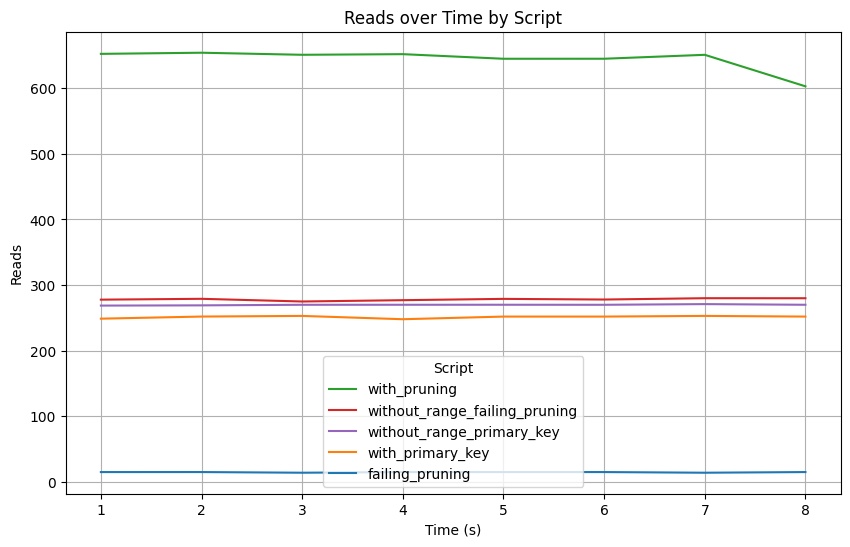
\includegraphics[width=\textwidth]{PNGs/Script/Partition/range-partition/Reads}
		\label{range-partition-reads}
	\end{subfigure}
	\hfill
	\begin{subfigure}[t]{0.48\textwidth}
		\centering
		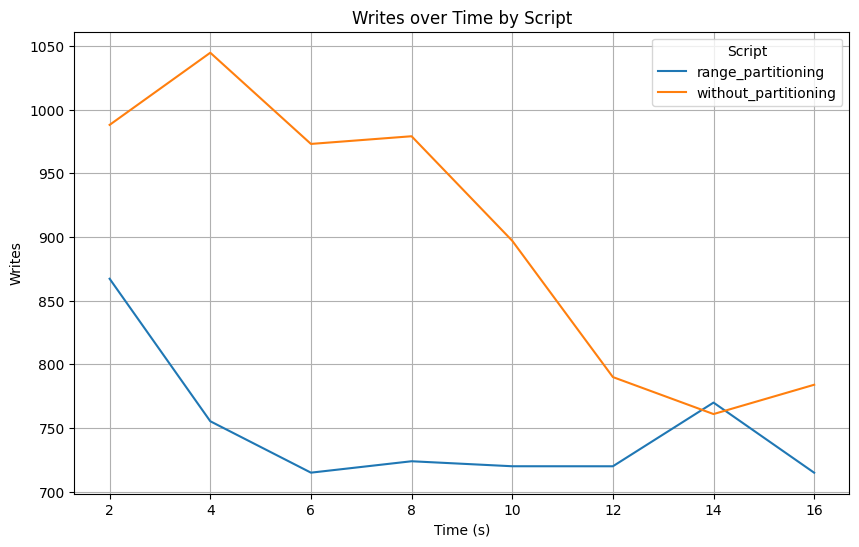
\includegraphics[width=\textwidth]{PNGs/Script/Partition/range-partition/Writes}
		\label{range-partition-writes}
	\end{subfigure}
	\vspace{-20pt}
	\caption[Range-Partitionierung: Metrikvergleich]{Vergleich zwischen der Range-Partitionierung und ohne Partition}
	\label{fig:range-partition}
\end{figure}
\vspace{-20pt}

Bei der List-Partitionierung~\ref{fig:list-partition} können wir auch einige interessante Beobachtungen machen.
Beim ersten Fall ist nur ein Land in der WHERE-Bedingung vorhanden.
Wenn dies so ist, dann hat die Partitionierung einen erheblichen Vorteil gegenüber der Version ohne Partitionierung (siehe rote Linie von with\_pruning\_simple und braune von without\_list\_pruning\_simple).
Wenn wir statt nur eines Landes mehrere abfragen, sehen wir für die verschiedenen Operatoren unterschiedliche Ergebnisse.
Die beste Performance erzielt der IN-Operator.
Dicht darauf folgt der OR-Operator.
Mit etwas größerem Abstand liegt der Fall ohne Partitionierung.
Deutlich abgeschlagen ist die Verbindung der Ergebnisse per UNION-Operator.
Die Performance beim Einfügen der Daten ist bei der Partitionierung und dem Referenzfall sehr ähnlich, wobei letzterer einen ganz leichten Vorteil hat.

\vspace{-8pt}
\begin{figure}[H]
	\centering
	\begin{subfigure}[t]{0.48\textwidth}
		\centering
		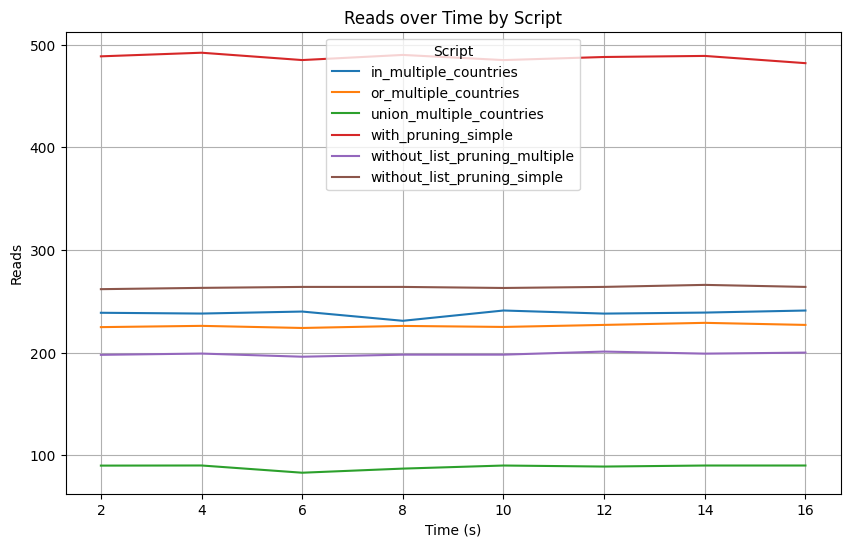
\includegraphics[width=\textwidth]{PNGs/Script/Partition/list-partition/Reads}
		\label{list-partition-reads}
	\end{subfigure}
	\hfill
	\begin{subfigure}[t]{0.48\textwidth}
		\centering
		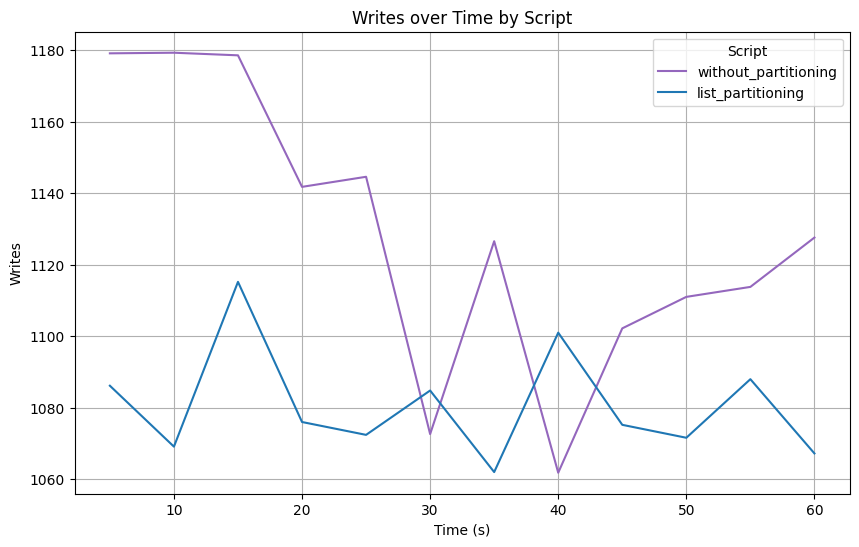
\includegraphics[width=\textwidth]{PNGs/Script/Partition/list-partition/Writes}
		\label{list-partition-writes}
	\end{subfigure}
	\vspace{-20pt}
	\caption[List-Partitionierung: Metrikvergleich]{Vergleich zwischen der List-Partitionierung und ohne Partition}
	\label{fig:list-partition}
\end{figure}
\vspace{-20pt}

Bei der Key-Partitionierung fällt auf, dass es keinen signifikanten Performance-Unterschied zur Hash-Partitionierung gibt, wenn derselbe Datensatz und dieselbe Anzahl von Partitionen verwendet wird.
Generell ist die Key-Partitionierung häufig stabiler und optimierter ist, insbesondere wenn es um Primärschlüssel geht.

Bei der Hash-Partitionierung~\ref{fig:hash-partition} nehmen sich beide Select-Fälle kaum etwas.
Auch hier fällt auf, dass die Werte der Abfragen sehr konstant sind.
Nur bei der Variante mit 500 Partitionen gibt es deutlich sichtbare Schwankungen.
Diese liegen aber nicht an dem Pruning, denn mit dem SQL-Befehl \texttt{EXPLAIN} sehen wir, dass alle 500 Partitionen benötigt werden und nicht keine Partitionen durch Zufall geprunt werden.
Die Hash-Partitionierung berechnet aus dem Wert einer bestimmten Spalte mithilfe einer Hash-Funktion einen Hash-Wert und anhand dessen wird die Zeile einer der Partitionen zugewiesen.
Da der Hash-Wert bei 500 Partitionen mit modulo 500 gebildet wird, landet jeder 500.\ Wert in der gleichen Partition.
Damit ist klargestellt, dass immer alle Partitionen benutzt werden, was die folgenden Ergebnisse zeigen.
Zunächst zeigt sich, dass die Abfrage ohne Partitionierung am schnellsten ist.
Danach kann man der Regel, dass je mehr Partitionen es gibt, desto langsamer wird die Query.
Der Unterschied zwischen ohne Partitionen und 5 Partitionen ist noch überschaubar, aber bei 500 Partitionen sieht man einen sehr deutlichen Unterschied.
Das bestätigt die wichtig von unserem Leitsatz, dass je mehr Partitionen benötigt werden, desto aufwendiger wird die Suche innerhalb der Partitionsstruktur, was die Performance verringert.

\vspace{-8pt}
\begin{figure}[H]
	\centering
	\begin{subfigure}[t]{0.48\textwidth}
		\centering
		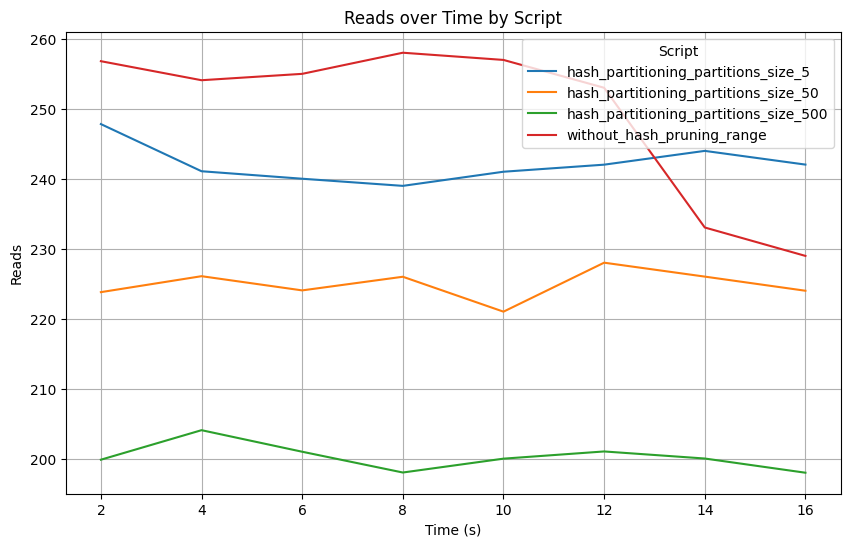
\includegraphics[width=\textwidth]{PNGs/Script/Partition/hash-partition/Reads}
		\label{hash-partition-reads}
	\end{subfigure}
	\hfill
	\begin{subfigure}[t]{0.48\textwidth}
		\centering
		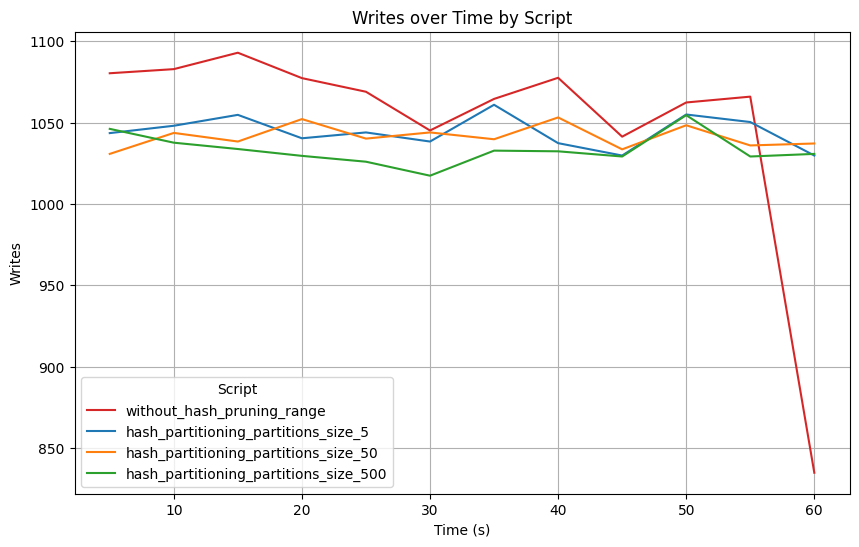
\includegraphics[width=\textwidth]{PNGs/Script/Partition/hash-partition/Writes}
		\label{hash-partition-writes}
	\end{subfigure}
	\vspace{-20pt}
	\caption[Hash-Partitionierung: Metrikvergleich]{Vergleich zwischen der Hash-Partitionierung und ohne Partition}
	\label{fig:hash-partition}
\end{figure}
\vspace{-20pt}